\documentclass[tikz,border=5pt]{standalone}
\usepackage{fontspec}
\setmainfont{Times New Roman}
\usepackage{unicode-math}
\setmathfont{Cambria Math}
\usetikzlibrary{shapes.geometric,shapes.misc,positioning,fit,backgrounds,arrows.meta,calc}

\begin{document}
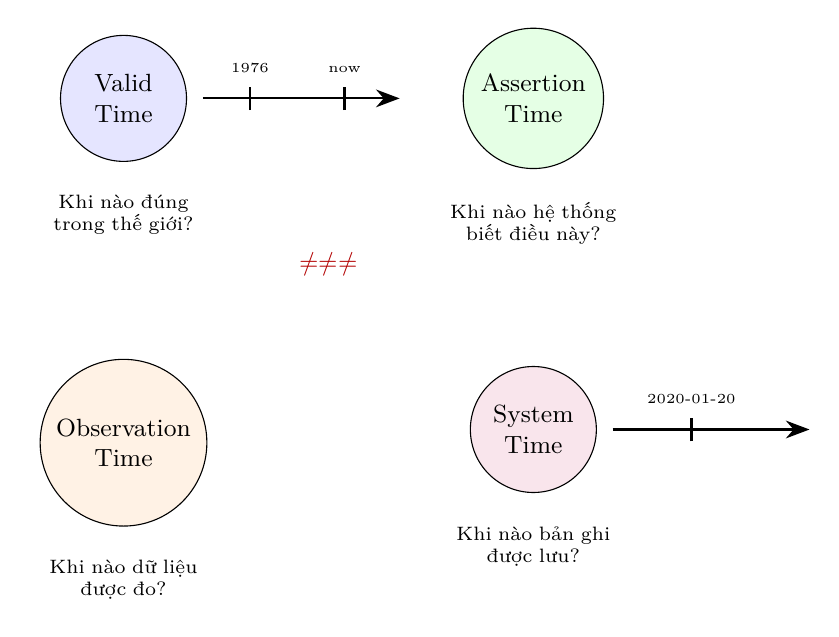
\begin{tikzpicture}[
    clock/.style={circle, draw, minimum size=1.6cm, align=center, font=\small},
    timeline/.style={thick, -{Stealth[length=3mm]}},
    lbl/.style={font=\scriptsize, align=center, text width=2.2cm},
]

% Four clocks arranged in 2x2 grid
\node[clock, fill=blue!10] (valid) {Valid\\Time};
\node[clock, fill=green!10, right=3.5cm of valid] (assertion) {Assertion\\Time};
\node[clock, fill=orange!10, below=2.5cm of valid] (observation) {Observation\\Time};
\node[clock, fill=purple!10, below=2.5cm of assertion] (system) {System\\Time};

% Questions each clock answers
\node[lbl, below=0.3cm of valid] {Khi nào đúng\\trong thế giới?};
\node[lbl, below=0.3cm of assertion] {Khi nào hệ thống\\biết điều này?};
\node[lbl, below=0.3cm of observation] {Khi nào dữ liệu\\được đo?};
\node[lbl, below=0.3cm of system] {Khi nào bản ghi\\được lưu?};

% Example timeline for valid time
\draw[timeline] ($(valid.east)+(0.2,0)$) -- ++(2.5,0);
\draw[thick] ($(valid.east)+(0.8,-0.15)$) -- ++(0,0.3);
\draw[thick] ($(valid.east)+(2.0,-0.15)$) -- ++(0,0.3);
\node[font=\tiny, above] at ($(valid.east)+(0.8,0.2)$) {1976};
\node[font=\tiny, above] at ($(valid.east)+(2.0,0.2)$) {now};

% Example timeline for system time
\draw[timeline] ($(system.east)+(0.2,0)$) -- ++(2.5,0);
\draw[thick] ($(system.east)+(1.2,-0.15)$) -- ++(0,0.3);
\node[font=\tiny, above] at ($(system.east)+(1.2,0.2)$) {2020-01-20};

% "NOT interchangeable" annotation
\node[font=\small\bfseries, text=red!70!black, anchor=center] at ($(valid)!0.5!(system)+(0,0)$) {$\neq \neq \neq$};

\end{tikzpicture}
\end{document}
